\subsubsection{ACI Visualization}
As ACI is best represented over a period of time, the first infographics that come to mind for representing it are line charts and histograms. A line chart would be able to represent ACI values over time and also represent multiple results across time. This benefits users because it allows them to visually compare results taken at the same time of day, but from different days. Our sponsor mentioned that being able to see if there is a correlation between time of day and when a site is loud or quiet is useful in research. A histogram on the other hand is best fit for representing the distribution of a single variable over time. This would be useful for representing a single result, instead of comparing results over time. Thus, the two visualizations initially available for ACI were line charts for comparing results, and a histogram for individual results.\\

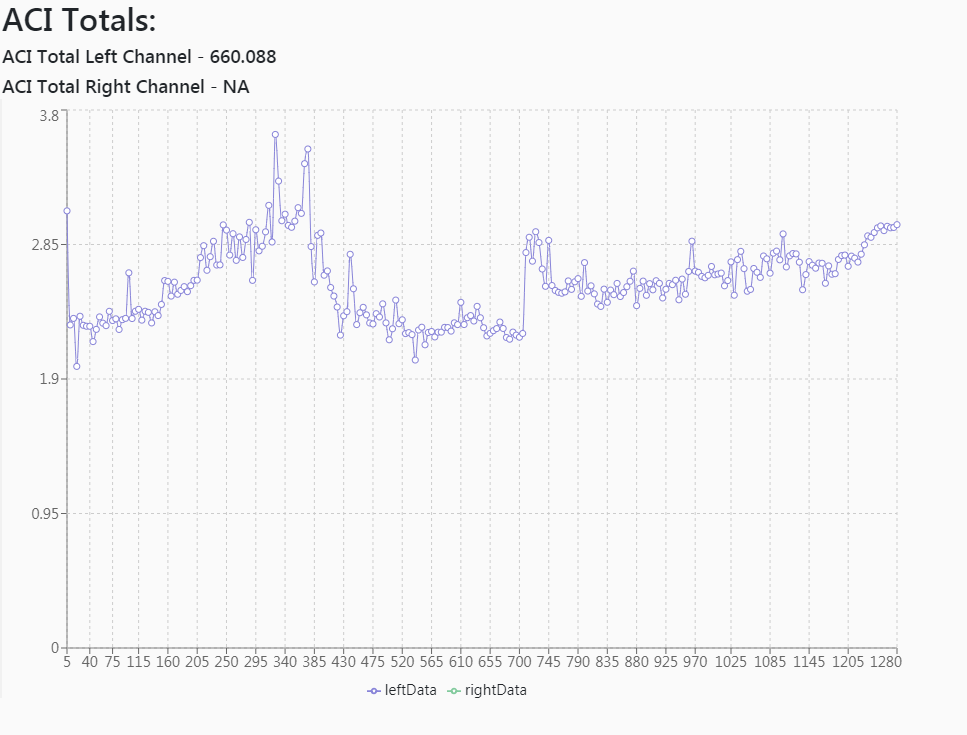
\includegraphics[width=\textwidth]{ACIgraph1}
This was the first idea for creating a visualization of ACI. This graph included the ability to see the specific value for each data point, which is useful for researchers. The X axis represents the time stamp in the file, and the Y axis represents the ACI value at that time stamp. The heading of the graph includes the ACI total value for both the left and the right channel. This graph is nice, however it does not include the ability to zoom into a specific time range, something that can be useful especially for longer files. Thus the next iteration came to fruition.\\

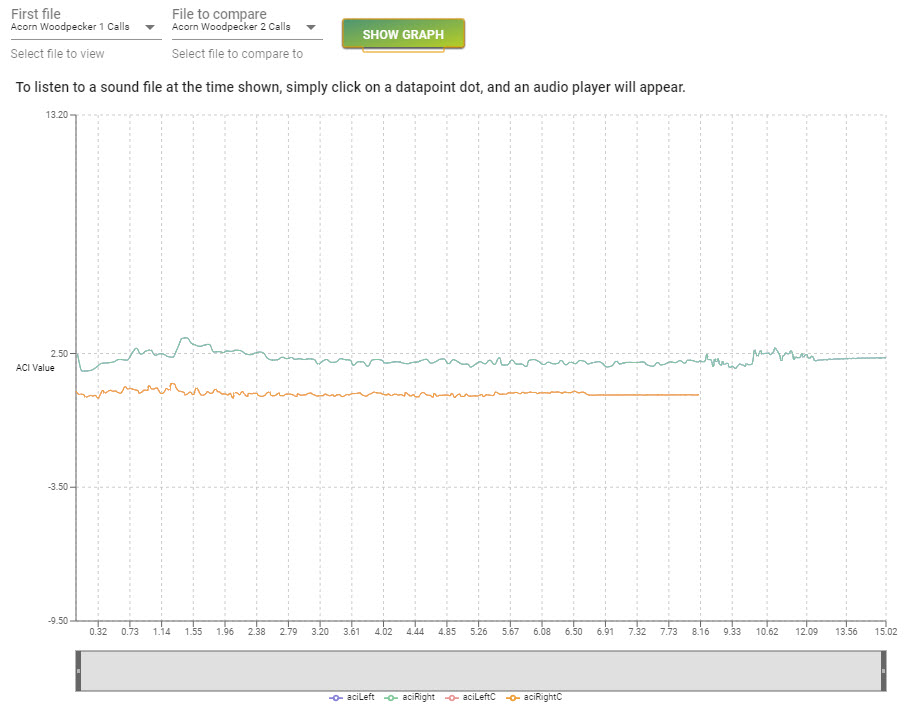
\includegraphics[width=\textwidth]{ACIgraph2}
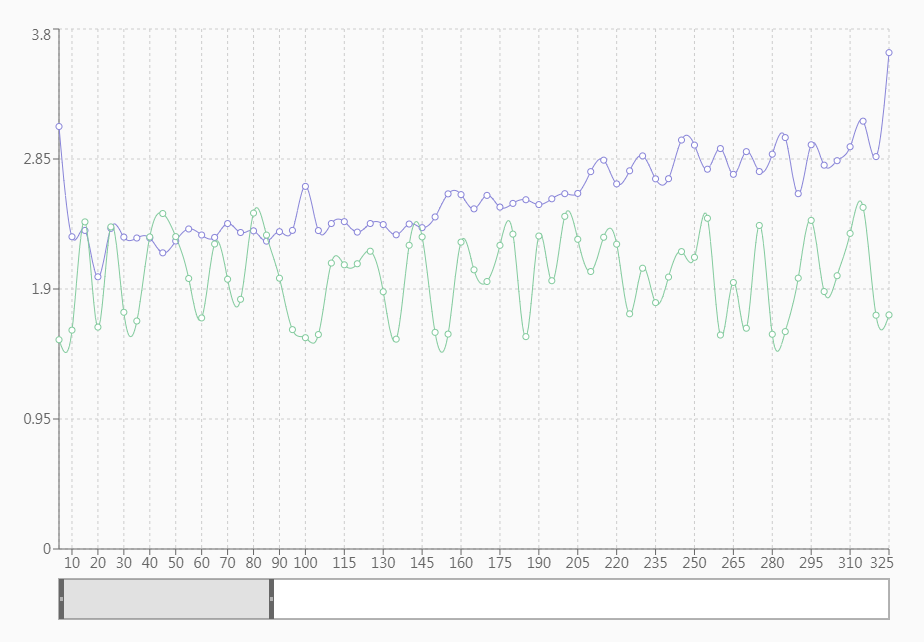
\includegraphics[width=\textwidth]{ACIgraph2-1}
These graphs are similar to the first version, however they include a brush bar. This bar can be used to specify a range of time that the graph natively zooms in on, as shown in the second image. In addition, that range of time can be scrolled through, so the user could filter by thirty second intervals and manually scroll through the data as they please. We feel this visualization is the best representation for both the data and the user.\\
